\documentclass[10pt,a4paper]{article}
\usepackage[utf8]{inputenc}
\usepackage{amsfonts}
\usepackage{graphicx}
\usepackage[margin=1.2in]{geometry}
\usepackage{multirow}
\usepackage[parfill]{parskip}
\usepackage{float}
\usepackage[justification=centering]{caption}
\usepackage{pifont}
\usepackage[table]{xcolor}
\newcommand{\cmark}{\ding{51}}
\newcommand{\xmark}{\ding{55}}

\title{ EDIC report \\ \large Mem0r1es extraction from browser activities}
\author{Jean-Eudes Ranvier\\\texttt{jean-eudes.ranvier@epfl.ch}}


\begin{document}
\sloppy

\maketitle

\section{Introduction}
In \textit{"Google effects on memory: Cognitive consequences of having information at our fingertips"} \cite{sparrow2011google}, Sparrow et al.~show that, more and more, people turn to their computers when confronted with something they don't know. However, the quantity of information that can be found on Internet has been increasing at an incredibly fast pace for the last decade, and as a natural consequence users are browsing through more and more information every day. We believe that users often look for information they already looked up in the past and therefore favor retrieving information from their ``closed world'' (i.e. every pages he already visited) rather than from the ``open world'' (i.e. the whole world wide web). However, while the Web search engines still improve at fast pace, the tools available to retrieve information from one's ``closed world'' remain too basic.

This project exploits the APIs that modern browsers provide to extract not only the pages visited by the user, but also an extensive set of relevant features. We believe that such features would improve the information retrieval within the digital memories that a user constructs from her browsing activity. For this reason, we have built a framework which enables simple IR tasks within the digital memory. Such fremework can be used as a cornerstone to enable more advanced tasks: e.g., we are currently performing a joint experiment with neuroscientists (from the laboratory of cognitive neuroscience [LNCO]) of EPFL which proposes to study the memorization process underlying Web browsing activity.

The remainder of this paper is organized as follows: In section~\ref{sec:relatedWork}, we overview the related work. In section~\ref{sec:architecture} we give some key insights on the architecture of the framework while in section~\ref{sec:implementation} we provide some details about the implementation and we evaluates its performance. In section~\ref{sec:evaluation}, we describe the user study planned conjointly with the LNCO laboratory and finally, in section~\ref{sec:conclusion} we conclude our work and provides some future steps orientation.
%#############

\section{Related Works}
\label{sec:relatedWork}
There is significant amount of systems dealing with collecting and indexing personal information from the Web, some mature systems are already in use. The most trivial of this system is the browser history itself which provide the user with a simple time ordered list of pages she already visited. However the number of features that this system provides is limited. For instance, very few systems record the user activity on web pages while this feature might give important insight about what the user highlited and found important.

One tool to extract information about a Web page is to use a toolbar \cite{white2010assessing} \cite{guo2010ready} \cite{hassan2012task} \cite{kotov2011modeling} which gather additional information such as the language of the page and the referrer (i.e.  the address of the webpage that linked to the resource). It is also well suited for studies of multiple users since this data can be extracted from well known toolbars and then centralized. Another broadly used approach in the literature is server logs \cite{donato2010you} \cite{west2012human} \cite{agichtein2012search}. Indeed, this method does not require any interaction with the user while providing useful information such as the timestamp, URL served and the referrer of the page which allow browsing session reconstruction. But this approach has also the inconvenience to be limited to the pages that the server actually serves, hence making it more application specific. A related project conducted by Microsoft Research \cite{kramardetecting} makes use of a proxy to track every page visited by the user and uses the proxy to inject a Javascript script on every pages in order to track user's activity on the page and the amont of time he spent on it. A processing of the pages allows them to extract semantic information such as keywords, tags and named entities as well as a categorization of the page against an ontology. Closer to our concerns, the Archify software \cite{archify} is designed as a browser extension which gather the user's browsing history along with some additional information such as the location from which the browsing happened, the referrer of each page, the time spent on pages, as well as a strong integration with well known online social networks such as Facebook, Twitter and LinkedIn. The extension then stores this information online to make them available from everywhere.

%#############

\section{Architecture}
\label{sec:architecture}

In light of the features extracted by the different systems described in the previous section, we define a list of features to extract in order to obtains as much information about the content of the page or the context in which it has been visited.

{\renewcommand{\tabcolsep}{0.1cm}
\begin {table}[H]
\begin{center}
\begin{tabular}{|l|c|c|c|c|c|c|}
\hline
\multicolumn{1}{|c|}{\textbf{feature}}& \textbf{mem0r1es} & \textbf{browser history} & \textbf{toolbar} & \textbf{server logs} & \textbf{archify} & \textbf{proxy} \\
\hline
url & \cmark & \cmark & \cmark & \cmark & \cmark & \cmark\\
title & \cmark & \cmark & \xmark & \xmark & \cmark & \xmark\\
content & \cmark & \xmark & \xmark & \xmark & \cmark & \xmark\\
language & \cmark & \xmark & \cmark & \xmark & \xmark & \xmark\\
referrer & \cmark & \xmark & (\cmark) & (\cmark) & \cmark & \xmark\\
timestamp & \cmark & \cmark & \cmark & \cmark & \cmark & \cmark\\
user activity & \cmark & \xmark & \cmark & \xmark & \xmark & \cmark\\
screenshot & \cmark & \xmark & \xmark & \xmark & \cmark & \xmark\\
page focus & \cmark & \xmark & \xmark & \xmark & \xmark & \cmark\\
context & \cmark & \xmark & \xmark & \xmark & (\cmark) & \xmark\\
semantic analysis & (\cmark) & \xmark & \xmark & \xmark & \xmark & \cmark\\
social integration & (\cmark) & \xmark & \xmark & \xmark & \cmark & \xmark\\
\hline
\end{tabular}
\end{center}
	\caption{ Comparison of the capacities of the mem0r1es extension against other approaches from the literature (\cmark : extracted , \xmark: not extracted, (\cmark): can be potentially extracted)}
	\label{table:relatedProjects}
\end {table}
}

Our system relies on a browser extension to extract relevant information from the browsing activity of the user.

\begin{figure}[h!]
 \centerline{
 	 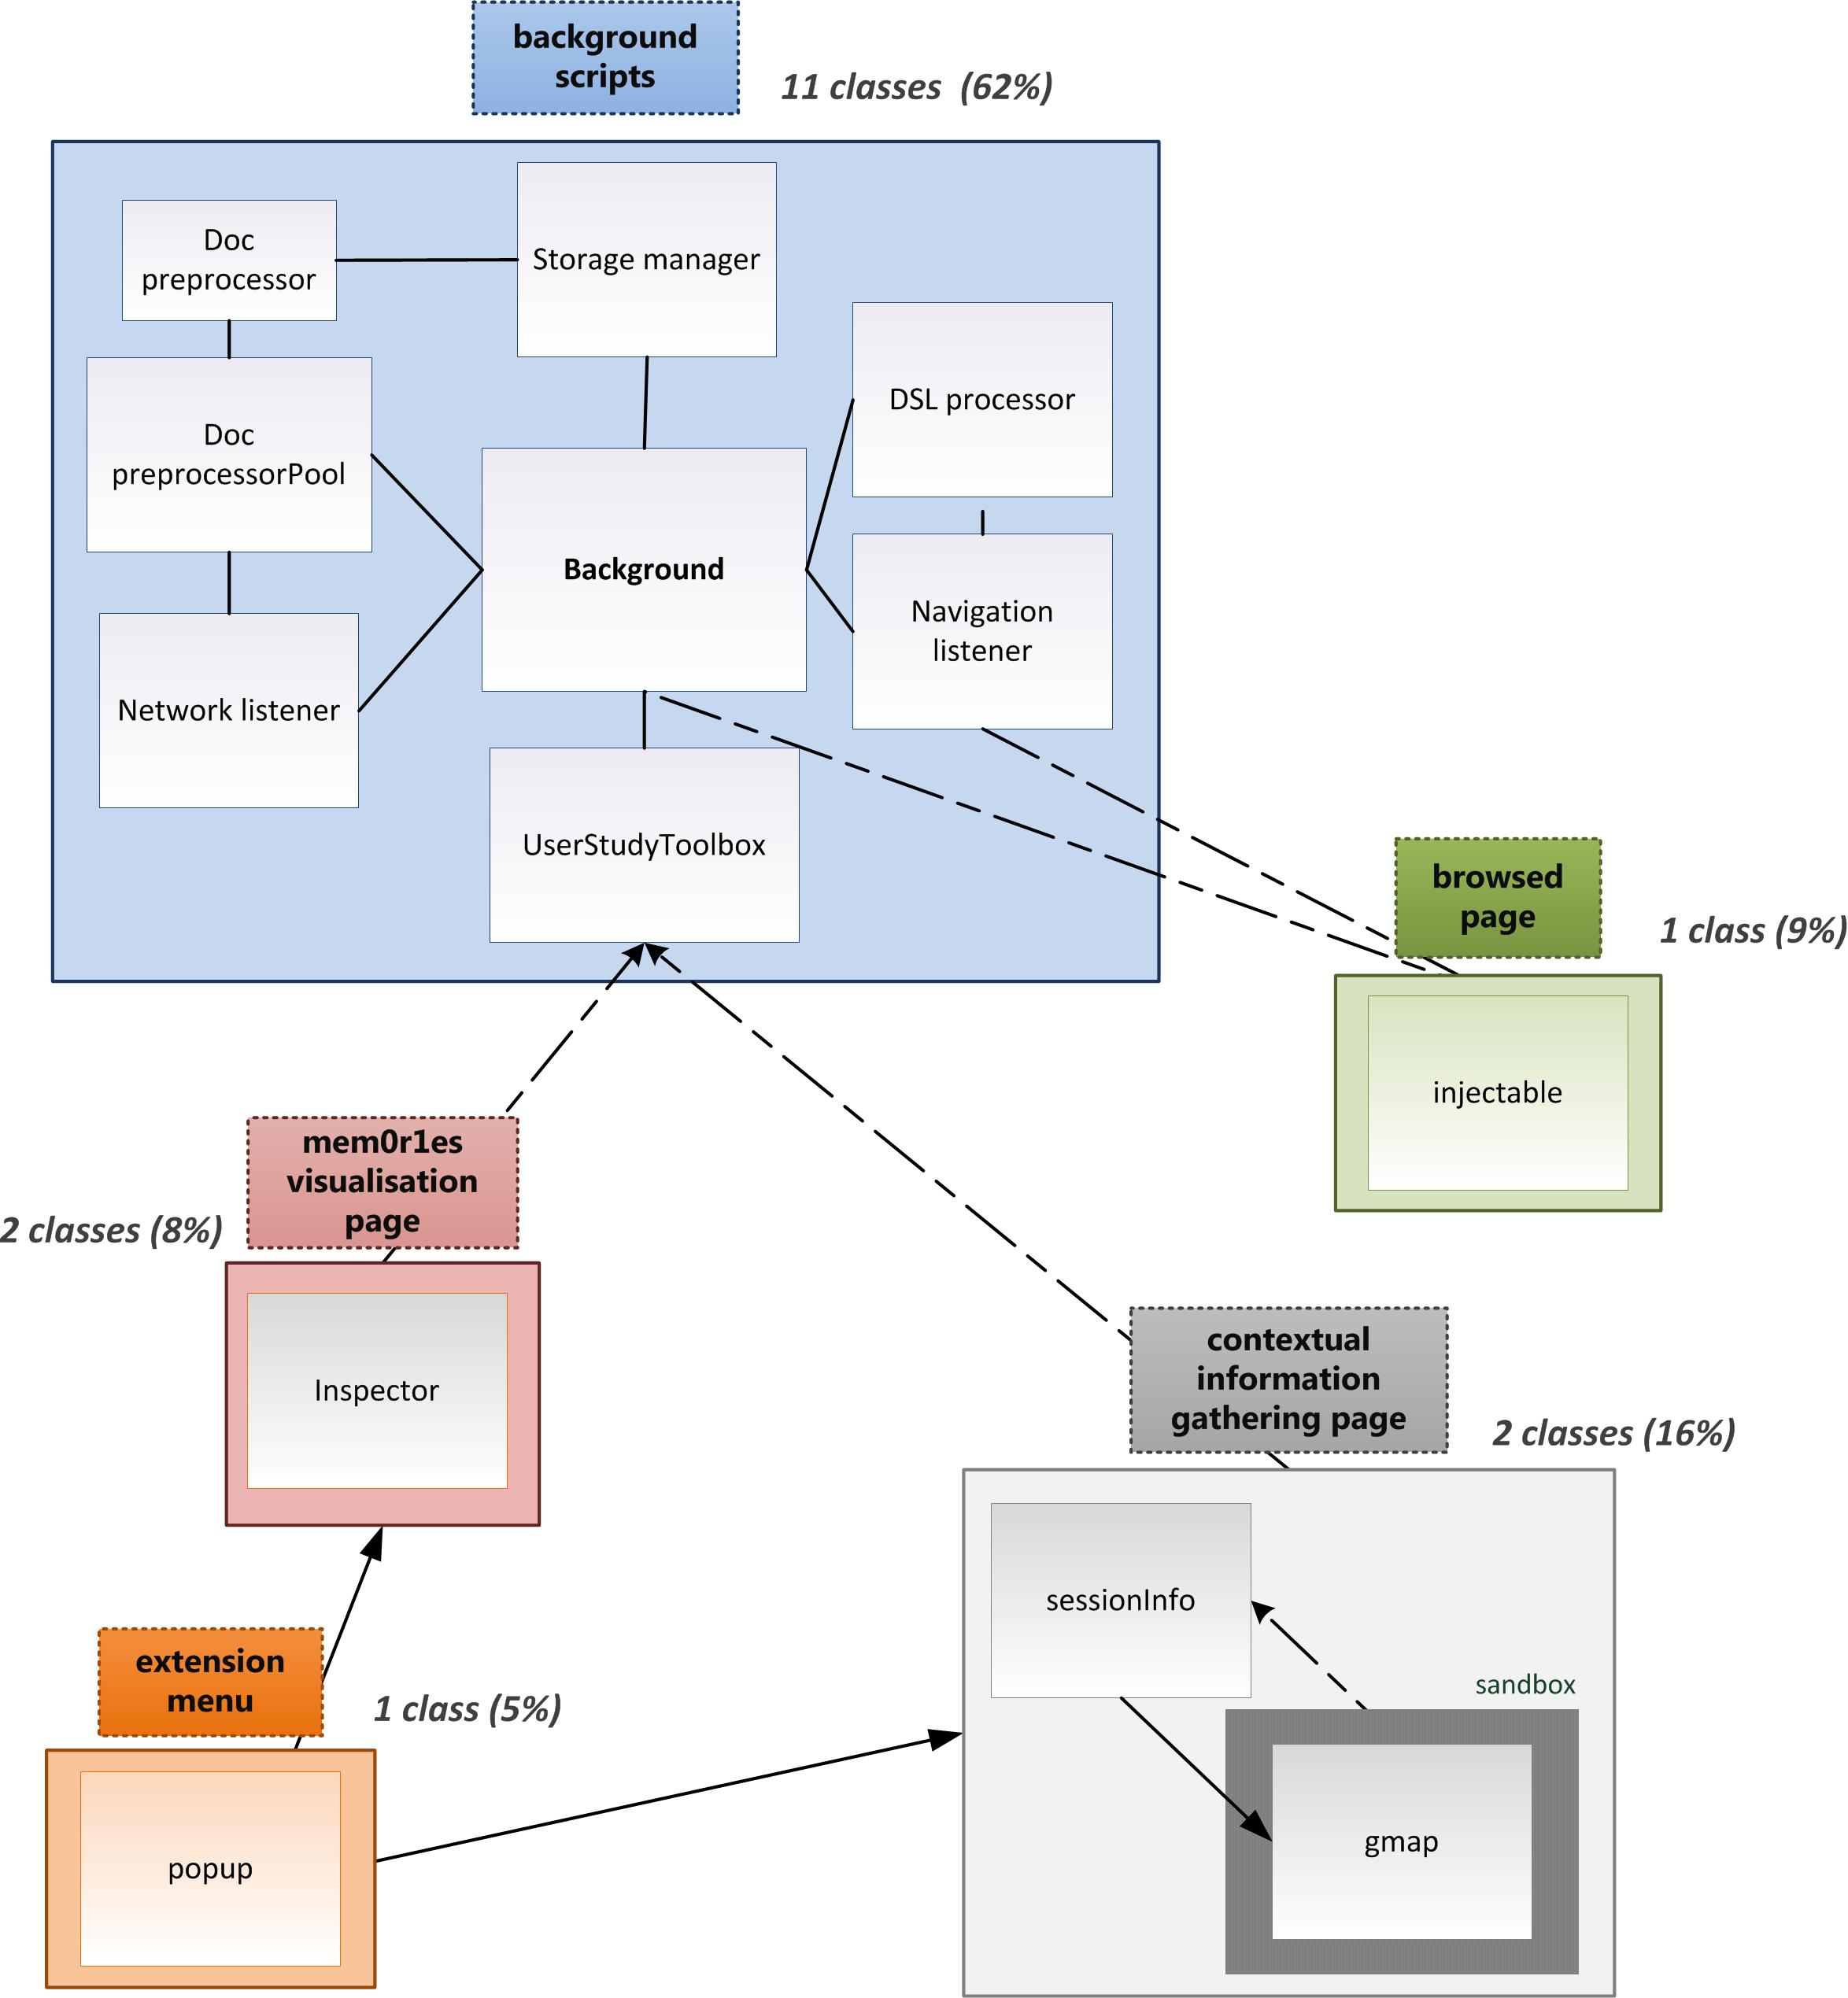
\includegraphics[width=0.8\textwidth]{figures/architecture.jpg}}
 \caption{ Class diagram of the extension divided by components with there respective number of classes (and the percentage of line of code they represent)}
\label{fig:architecture}
\end{figure}

\subsection{Data collection}
\label{subsec:dataCollection}
As depicted in figure~\ref{fig:architecture}, the extension is built around a background script which is executed when the browser starts. It is in charge of loading the different services such as the database manager and the network listener. Each page viewed by the user is processed to extract several information: its content, the actions the user took on this page, its language, the referrer of the page, a screenshot of the page, the time the page spend in the foreground. In addition to these features, some additional domain\footnote{In this context, \textit{domain} refers to the domain name of the website to which the page belongs} specific features can be extracted (e.g. the mouse moves of gaming website, the shopping basket of an online store, etc). This information is then stored using a data access object (DAO) which acts as an interface between the extension and the database system. As part of the user study described in section~\ref{sec:evaluation}, additional information about the browsing session is also collected. This information regards the context in which this session occurred and includes the time at which the it happened, a picture of the user and its labeled location.

\subsection{Data indexing}
\label{subsec:dataIndexing}
The data extracted by the extension is stored locally in indexedDB \cite{indexeddb}. This database allows to store hierarchical data in different object stores as a key value pair. However indexedDB does not allow any relational modeling. Therefore, in order to distribute the different elements that we gathered across several stores, we implemented a simple relational system directly in javascript. The figure~\ref{fig:database} defines the database schema and show the relations between the different object stores. While this mechanism is clearly less effective than what a relation system integrated directly at the database level could provide, it allows us to retrieve only part of a page information or to select pages from a browsing session. Please note that in figure~\ref{fig:database}, only the primary keys and indices are displayed. Since IndexedDB does not support schemas, any JSON object can be inserted in the object stores and only these indices are mandatory.
\begin{figure}[h!]
	\centerline{
		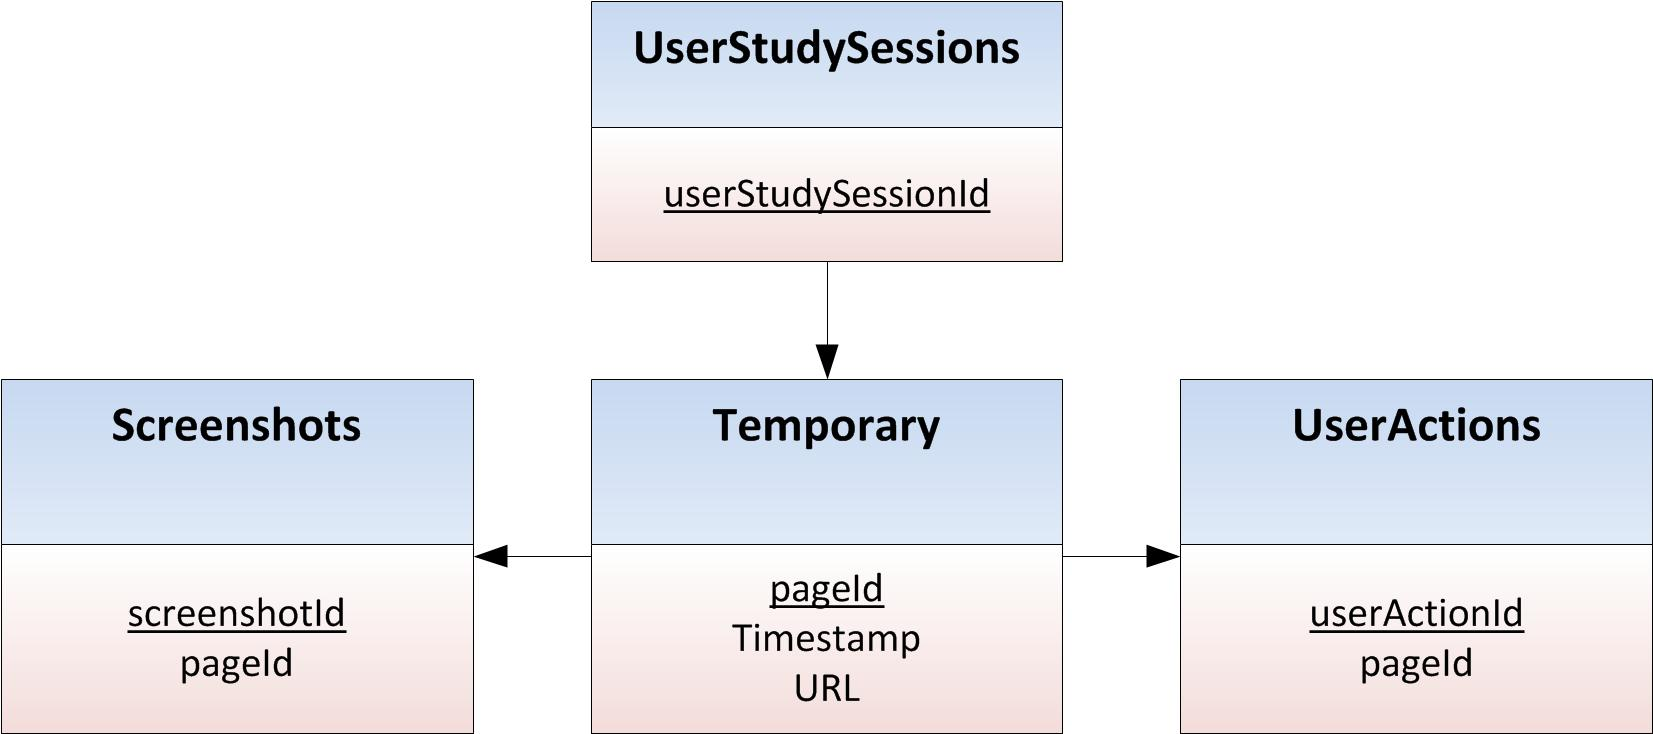
\includegraphics[width=0.5\textwidth]{figures/database.jpg}}
	\caption{ Database structure}
	\label{fig:database}
\end{figure}

\subsection{Privacy concerns}
As a browser extension, mem0r1es has access to every pieces of information that the user can read (or input) from (or in) the browser. This includes sensible and personal information (e.g. emails, online bank account pages, etc) which are critical for the user and should be handled with care. To address this privacy issue, the mem0r1es extension provides a variety of safety mechanisms.

The first protection comes from the fact that the data gathered by mem0r1es is stored in a local database, and can only be accessed from the extension. Indeed, Chrome sets each extension and each website in a different scope; rules to communicate between scopes have been strongly restricted in order to prevent third-party extensions or websites to access the data from our extension. Another mechanism is also provided by Chrome itself with its Incognito mode in which the extension is disabled. This means that any browsing done in Incognito mode will not leave any trace in the mem0r1es database. In addition to that, a custom Incognito mode has been created to prevent temporarily the recording of the browser activity.

The user study described in section~\ref{sec:evaluation} requires the centralization and the processing of users data. In order to respect the privacy of the participants, before sharing their data, they will be prompted with the possibility to blacklist some of these websites if they are not ready to share their activity on this website.

\section{Implementation}
\label{sec:implementation}
Its popularity, and its simplicity made Chrome the browser of choice to implement the extension. The implementation is done in CoffeeScript, an object-oriented language that compiles to javascript which is the default language for Chrome extensions. The user interface is created in HTML and, in order to accelerate the development and to observe good practices, we use third party libraries such as the bootstrap framework \cite{bootstrap} which  is used to build a clear user interface and the angularJs library \cite{angularjs} which is used to dynamically display the data to the user.


\subsection{Benchmarks}
In order not to disturb the browsing experience of the user, our Chrome extension should not have a significant impact on the loading time of pages or any other browser related activities. To evaluate such impact, two different Javascript benchmarks have been run both with the mem0r1es extension enabled and disabled.

The \textit{octane}\cite{octane}  benchmark runs a battery of tests designed to assess the performance of the browser in several Javascript use cases. We use this test to show that our extension does not have any impact on the browsing of a single page. The results of octane are available in table~\ref{table:octane}. The scores obtained with or without the extension are similar, the difference between them is most likely coming from processes started by the underlying operating system, independently of the browser.
\begin {table}[H]
\begin{center}
\begin{tabular}{|c|c|c|}
	\hline
	\multirow{2}{*}{\textbf{Iteration}} & \multicolumn{2}{ c| }{\textbf{Score}}\\
	\cline{2-3}
 	 & without extension & with extension \\
	\hline
	1 & 10810 &11975 \\
	2 & 11703 &11683 \\
	3 & 11805 &10926 \\
	\hline
	\textbf{Average} & \textbf{11439} & \textbf{11528} \\
\hline
\end{tabular}
\end{center}
	\caption{ Results of the Octane benchmark (the higher the better) ran on a browser with and without the mem0r1es extension loaded}
	\label{table:octane}
\end {table}

Since the extension performs its intensive tasks mainly during page loading, we ran a second benchmark suite which loads programmatically and repeatedly a list of websites. \textit{Page benchmarker} \cite{pageBenchmarker} allows us to load a list of websites and records the loading time. Therefore, the difference between the benchmark ran with and without the extension loaded it gives the time overhead generated by the extension. The benchmark uses three websites which are opened and closed 50 times:

\begin{itemize}
	\item \textit{www.epfl.ch} To measure the impact of the extension on local pages (i.e. a very low network overhead)
	\item \textit{mail.google.com} To measure the impact on heavy pages (i.e. which contains complex Scripts)
	\item \textit{twitter.github.com/bootstrap/components.html} To measure the impact on long pages (i.e. which contains an important DOM)
\end{itemize}

The results, displayed in table~\ref{table:pageBenchmarker}, show an overhead of around 10\% on a "local" page which represents 48 milliseconds. They also indicate that the network fluctuations as well as the serving time on the server side in the case of the Google and Github pages absorbs the impact of the mem0r1es extension.

The two presented benchmarks determine the impact of the mem0r1es extension on the browsing experience, showing that it does not affect it significantly. We can notice that the \textit{page benchmarker} benchmark imposes a stress on the system which is way higher than the one from a normal usage, but the extension can still handle it without problems.

\begin {table}[H]
\begin{center}
\begin{tabular}{|l|c|c|c|c|}
\hline
\multicolumn{1}{|c|}{\multirow{2}{*}{\textbf{Website}}} & \multicolumn{2}{ c| }{\textbf{Average loading time}} & \multicolumn{2}{ c| }{\textbf{Overhead}} \\
\cline{2-5}
& without extension & with extension & relative & absolute\\ 
\hline
www.epfl.ch & 545.8 & 593.8 & 8.8\% & 48\\
mail.google.com & 2190.3 & 2283.3 & 4.2\% & 93\\
twitter.github.com/b...nents.html & 2135 & 1914.5 & -10.3\% & -220.5\\
\hline
\end{tabular}
\end{center}
	\caption{ Results of the pageBenchmarker benchmark (in ms) ran on a browser with and without the mem0r1es extension loaded}
	\label{table:pageBenchmarker}
\end {table}


%#############

\section{Ongoing Evaluation}
\label{sec:evaluation}

In order to evaluate which are the prominent features influencing the memorization process, we are jointly working with a team of neuroscientists from LNCO on a user study which should give some insights about this process.

Kristo et al. in \cite{kristo2009retention} define a user study which aims at detecting the important factors in the retention of autobiographical memories. To this purpose, in the first place he asks each participant of the study to describe a specific personal event. The author defines several features of this event for which the participant has to provide information such as \textit{what was the event?}, \textit{who was involved?}, \textit{where it happened?}, \textit{when it happened?}. All this information is used as a set of cues for the second part of the experiment which take place after 2 to 46 days. In this second step, the participant has to answer again one of the question he previously answered. She is provided with the right answer and then asked about a second feature, et cetera until she answered all the question about the event. By asking the questions in a random order, Kristo defines which of the features play an important role in the memorization process.

However by openly asking the participants to provide all the information in a first place, such study is relatively overt toward the participants, which may lead to biased results. To avoid this problem we plan to record \textit{automatically} the browsing activity of the participants for one full week along with some contextual information such as pictures of the user and location information. At the end of a retention period of one extra week, we plan to run two separate experiments. Both of them are recognition tasks in which the user will be presented with data she will have produced or some manipulated data. The manipulations are of that form: The picture, the location of the user as well as the time at which the page was visited are contextual data and can be swapped with an equivalent feature from another browsing session. The page can be seen as bearing a content (i.e. the actual information) as well as a context (e.g. the appearance of the page). Therefore its manipulation should be made along these two axis. Table~\ref{table:pageManipulation} lists the different manipulations that can be done and gives example of website which are well suited for each cases.

\begin {table}[H]
\begin{center}
\begin{tabular}{|m{2.8cm}|m{3cm}|m{7cm}|}
\hline
\multicolumn{1}{|c|}{\textbf{manipulation}} &\multicolumn{1}{|c|}{\textbf{websites used}}&\multicolumn{1}{|c|}{\textbf{explanation}}\\
\hline
same content \newline same context & news websites \newline scientific platforms \newline wikipedia & the page that she actually visited (no manipulation) \\
\hline
different content \newline same context & news websites \newline scientific platforms \newline wikipedia & a page that she did \textbf{not} visit but which is closely related to the page she actually visited\\
\hline
same content \newline different context  & news websites \newline scientific platforms & a page from another news website but about the news that she read \\
\hline
\end{tabular}
\end{center}
	\caption{Manipulation of a page based on its content or context}
	\label{table:pageManipulation}
\end {table}


\subsection{First experiment - explicit}
In the first experiment we will investigate how good people are at remembering the pages they visited as well as the contextual information associated with those pages. We will also compare their actual memory abilities with their subjective confidence about their memories.

In a first step, the user will be asked, how good she thinks she remembers a page she visited one of the four dimensions listed in table~\ref{table:dimensions}. This initial evaluation is used as an a priori and self-assessed estimation of the user memorization ability.

In a second step, each of these dimensions will be tested separately. The user will be provided sometime with original memories of pages she visited and sometime with mem0r1es manipulated according to the manipulations defined at the beginning of the section. For each of these memories the user will be asked one of the typical questions defined in Table~\ref{table:dimensions}. The user will also be asked to provide her confidence about her answers on a continuous scale.

\begin {table}[H]
\begin{center}
\begin{tabular}{|l|l|}
\hline
\multicolumn{1}{|c|}{\textbf{Dimension}} &\multicolumn{1}{|c|}{\textbf{Typical question}}\\
\hline
Page itself &  Do you remember having visited this page?\\ 
\hline
Physical aspect of the user & When you visited this page, did you look like that?\\
\hline
Time & When you visited this page, was it at that day/time?\\ 
\hline
Place & When you visited this page, were you at that place?\\ 
\hline
\end{tabular}
\end{center}
	\caption{ Dimensions queried in the experiment and their related question}
	\label{table:dimensions}
\end {table}

\subsection{Second experiment - implicit}
In the second experiment, we will investigate whether contextual information associated to a specific web-browsing experience automatically boosts memory for the content of this browsing experience. This experiment will be run on a different set of users than the first one and will be defined as follow:

The user is presented with a piece of contextual information. After making sure that the user saw the clue, she is presented with a page and is asked if she visited it. By mixing congruent pairs (i.e. contextual pieces of information belonging to the session in which the user has seen the page) and incongruent pairs, we will see which type of clue helps the user to remember if she visited a page and which do not.

\subsection{Origin of information discovery}
From the data gathered for the two experiments described above, a third experiment can be run on the importance of social networks regarding information discovery. We argue that users might show different memorization behavior when they are exposed to new content through online social networks (e.g., Facebook, Twitter, etc.), rather than standard vertical websites (e.g., online newspapers, technology websites, etc.)

To run such study, we will rely on the referrer functionality exploited by most websites to track user provenance in browsing sessions. That is to say, when a user is clicking on a link she just saw on Twitter, the destination website will know that she didn’t discover the news article by chance, but she has been brought there by a Twitter link. Given that we record most of the browsing activities, we also have the Referrer available for every page visited. 


\section{Conclusions}
\label{sec:conclusion}
With more and more user applications converging to the Web, Internet browsers are becoming a goldmine when it comes to user behavior studies. Targeted advertising and e-commerce recommendations already proved the economical value of carefully tracking the activities of a user on the Web. With this project, we assessed how modern browsers can be exploited to obtain even more information, while preserving the data privacy oftentimes violated by third-party trackers. When compared to previous works, the proof-of-concept we have built proves how the careful usage of advanced browser APIs can indeed elicit a superset of the commonly extracted features. At the same time, our extension enables a variety of new user study scenarios. For the scope of the project, we focused on assessing what is memorable (and forgettable) for an Internet user, to get a glimpse of how human memory works. As a future step, we are already exploring solutions to enhance the browser history from a trivial, time-ordered list of URLs, to a tool that reflects carefully the specific characteristics of the human memory.

\section*{Acknowledgments}
I would like to express my gratitude to Michel Catasta with whom I'm working on this project. His precious advices are really helpful and his good mood always motivating. I also would like to thank Jean-Paul Noel and Andrea Serino from the LNCO laboratory for their patience while explaining basic neuroscience concepts and I finally would like to thank professor Karl Aberer for giving me the opportunity to do this semester project at the LSIR laboratory.

\begin{appendix}
\bibliographystyle{ieeetr}
\bibliography{references}
\end{appendix}	

\end{document}
